% Uncomment this to make slides with overlays:
%\documentclass[slides]{beamer}

% Uncomment these (but comment the above \documentclass line) to make handouts:
\documentclass[handout]{beamer}

% Uncomment these to have more than one slide per page
\usepackage{pgfpages}
\pgfpagesuselayout{2 on 1}[border shrink=5mm]
\pgfpageslogicalpageoptions{1}{border code=\pgfusepath{stroke}}
\pgfpageslogicalpageoptions{2}{border code=\pgfusepath{stroke}}

\usepackage[]{graphicx, color, hyperref}

\mode<presentation>
{
	%\usetheme[secheader]{Boadilla}
	%\usecolortheme[rgb={.835, .102,.169}]{structure}  
	\usetheme[width= 0cm]{Goettingen}
	%\setbeamercovered{transparent}
}
\setbeamertemplate{navigation symbols}{}
\setbeamertemplate{footline}[frame number]

\definecolor{blue2}{rgb}{0.278,0.278,0.729} 
\newcommand{\blue}[1]{\textcolor{blue2}{#1}}
\newcommand{\white}[1]{\textcolor{white}{#1}}
\newcommand{\red}[1]{\textcolor{red}{#1}}
\newcommand{\xbar}{\overline{x}}
\newcommand{\ybar}{\overline{y}}
\newcommand{\phat}{\widehat{p}}
\newcommand{\prob}{\mbox{Pr}}
\newcommand{\E}{\mathbb{E}}
\newcommand{\Var}{\mbox{Var}}
\newcommand{\cp}{\oplus}
\newcommand{\cm}{\circleddash}


\title{Lecture 21: Difference of two proportions}
\author{Chapter 6.2}
\date{}


\begin{document}
%------------------------------------------------------------------------------
\begin{frame}
\titlepage
\end{frame}
%------------------------------------------------------------------------------


%------------------------------------------------------------------------------
\begin{frame}
\frametitle{Previously... Proportions}

If
\begin{itemize}
\pause\item The sample observations are independent
\pause\item The \blue{success-failure condition} holds:
\begin{itemize}
\item $np \geq 10$
\item $n(1-p) \geq 10$ 
\end{itemize}
\end{itemize}
\pause then the sampling distribution of $\phat$ is nearly normal and hence we can:
\begin{itemize}
\item construct confidence intervals using $z^*$
\item conduct hypothesis tests and compute $p$-values using z-tables
\end{itemize}

\end{frame}
%------------------------------------------------------------------------------


%------------------------------------------------------------------------------
\begin{frame}
\frametitle{Previously... Proportions}

Both
\begin{itemize}
\pause\item to verify success/failure conditions
\pause\item in estimate of SE
\end{itemize}
we require an estimate of the true proportion $p$.  For
\begin{itemize}
\pause\item confidence intervals: use \blue{sample proportion $\phat$} in place of $p$
\pause\item hypothesis tests: use \blue{null value $p_0$} in place of $p$
\end{itemize}

\end{frame}
%------------------------------------------------------------------------------


%------------------------------------------------------------------------------
\begin{frame}[fragile]
\frametitle{Question for today}

How do we infer about a difference in proportions $p_1-p_2$?

\end{frame}
%------------------------------------------------------------------------------


%------------------------------------------------------------------------------
\begin{frame}[fragile]
\frametitle{Confidence Interval: Example from Text}

The way a question is phrased in survey can influence a person's response.  Ex:  the Pew Research Center conducted a survey with the following question:

\pause\vspace{0.5cm}

As you may know, by 2014 all Americans will be required to have health insurance.  \blue{X while Y}.  Do you approve of disapprove of this policy?

\pause\vspace{0.5cm}

where $X$ and $Y$ were randomly ordered between
\begin{itemize}
\item People who do not buy insurance will pay a penalty
\item People who cannot afford it will receive financial help from the government
\end{itemize}

\vspace{0.5cm}

\pause Build a 90\% confidence interval for the difference in proportions.  

\end{frame}
%------------------------------------------------------------------------------


%------------------------------------------------------------------------------
\begin{frame}[fragile]
\frametitle{Example from Text}

\begin{small}
\begin{center}
  \begin{tabular}{l|cccc}
     & Sample size & Approve & Disapprove & Other \\ 
     &  $n_i$ & (\%) & (\%) &  (\%)\\   
  \hline
    \blue{people who do not buy it}   & 771 & 47 & 49 & 3 \\ 
    \blue{will pay a penalty}  & &  &  &  \\ 
    given first & &  &  &  \\     
    \hline
    \blue{people who cannot afford} & 732 & 34 & 63 & 3 \\ 
    \blue{it will receive financial}  & & & &  \\ 
    \blue{help from the gov't} & & & &  \\ 
    given first & & & &  \\    
   \end{tabular}
\end{center}
\end{small}

\end{frame}
%------------------------------------------------------------------------------


%------------------------------------------------------------------------------
\begin{frame}[fragile]
\frametitle{Conditions for Sampling Dist'n of $\phat_1-\phat_2$ Being Normal}

When
\begin{itemize}
\pause\item both sample proportions $\widehat{p}_1$ and $\widehat{p}_2$ are approximately \blue{normal}:
\begin{itemize}
\item are independent
\item satisfies the success/failure condition from Lecture 9.1:  $np \geq 10$ and $n(1-p) \geq 10$
\end{itemize}
\pause\item the samples are independent from each other...
\end{itemize}

\end{frame}
%------------------------------------------------------------------------------


%------------------------------------------------------------------------------
\begin{frame}[fragile]
\frametitle{Conditions for Sampling Dist'n of $\phat_1-\phat_2$ Being Normal}

...the sampling distribution for the difference of sample proportions $\phat_1 - \phat_2$ is approximately normal with
\begin{itemize}
\pause\item mean $p_1 - p_2$
\pause\item standard error
\[
SE_{\phat_1 - \phat_2} = \sqrt{SE_{\phat_1}^2 + SE_{\phat_2}^2} = 
\sqrt{\frac{p_1(1-p_1)}{n_1} + \frac{p_2(1-p_2)}{n_2}}
\]
\end{itemize}
where $p_1, p_2$ are the true population proportions, and $n_1,n_2$ are the sample sizes.


\end{frame}
%------------------------------------------------------------------------------


%------------------------------------------------------------------------------
\begin{frame}[fragile]
\frametitle{Standard Error}

Recall when looking at numerical data, we showed that the SE for $\xbar_1-\xbar_2$ was
\[
SE_{\xbar_1-\xbar_2} = \sqrt{SE_{\xbar_1}^2 + SE_{\xbar_2}^2} = 
\sqrt{\frac{\sigma_1^2}{n_1} + \frac{\sigma_2^2}{n_2}}
\]
\pause Compare this to 
\[
SE_{\phat_1 - \phat_2} = \sqrt{SE_{\phat_1}^2 + SE_{\phat_2}^2} = 
\sqrt{\frac{p_1(1-p_1)}{n_1} + \frac{p_2(1-p_2)}{n_2}}
\]

\end{frame}
%------------------------------------------------------------------------------


%------------------------------------------------------------------------------
\begin{frame}[fragile]
\frametitle{Confidence Intervals}
Check the conditions:
\begin{itemize}
\pause\item Normality for each group
\begin{itemize}
\pause\item Each group is a sample random sample from less than 10\% of the population
\pause\item The success/failure condition holds for \blue{both} samples separately:
\begin{itemize}
\item $n_1\phat_1 \geq 10$ and $n_1(1-\phat_1) \geq 10$
\item $n_2\phat_2 \geq 10$ and $n_2(1-\phat_2) \geq 10$
\end{itemize}
\end{itemize}
\pause\item We assume both groups were sampled independently from each other.  
\end{itemize}

\end{frame}
%------------------------------------------------------------------------------


%------------------------------------------------------------------------------
\begin{frame}[fragile]
\frametitle{Confidence Intervals}
Point estimate is
\[
\phat_1 - \phat_2 = 0.47 - 0.34 = 0.13
\]

\pause Plug in $\phat_1$ and $\phat_2$ into SE:
\begin{eqnarray*}
SE_{\phat_1 - \phat_2} &=& 
\sqrt{\frac{\phat_1(1-\phat_1)}{n_1} + \frac{\phat_2(1-\phat_2)}{n_2}}\\
&=& \sqrt{\frac{0.47(1-0.47)}{771} + \frac{0.34(1-0.34)}{732}} = 0.025
\end{eqnarray*}

\end{frame}
%------------------------------------------------------------------------------


%------------------------------------------------------------------------------
\begin{frame}[fragile]
\frametitle{Confidence Intervals}

A 90\% confidence interval using the normal model is, as always:

\pause\begin{eqnarray*}
\mbox{point estimate} \pm z^* \times SE &=& \mbox{point estimate} \pm 1.65 \times SE\\
0.13 \pm 1.65 \times 0.025 &\Rightarrow& (0.09, 0.17)
\end{eqnarray*}

Since the confidence interval does not contain 0, 

\end{frame}
%------------------------------------------------------------------------------


%------------------------------------------------------------------------------
\begin{frame}[fragile]
\frametitle{Hypothesis Tests of $H_0: p_1=p_2$}
We are typically interested in differences in proportions being 0 vs something else.  For example
\begin{eqnarray*}
&&H_0: p_1 - p_2 = 0\\
\mbox{vs}&&H_1: p_1 - p_2 \neq 0
\end{eqnarray*}

\pause Note the null hypothesis can be re-expressed as $H_0: p_1 = p_2$.\\

\vspace{0.5cm}

\pause Thus, under the null hypothesis the two proportions are equal.  i.e. $p_1=p_2=p$

\end{frame}
%------------------------------------------------------------------------------


%------------------------------------------------------------------------------
\begin{frame}[fragile]
\frametitle{Hypothesis Tests of $H_0: p_1=p_2$}

So to
\begin{itemize}
\item verify the success-failure conditions
\item compute the standard SE
\end{itemize}
\pause we use a \blue{pooled estimate} $\widehat{p}$ of the proportion $p$
\[
\widehat{p} = \frac{\mbox{number of successes}}{\mbox{number of cases}} = \frac{\widehat{p}_1n_1 + \widehat{p}_2n_2}{n_1+n_2}
\]

\pause The estimate of the SE to use in for this hypothesis test is:
\[
SE_{\phat_1 - \phat_2} = \sqrt{\frac{\widehat{p}(1-\widehat{p})}{n_1} + \frac{\widehat{p}(1-\widehat{p})}{n_2}}
\]

\end{frame}
%------------------------------------------------------------------------------


%------------------------------------------------------------------------------
\begin{frame}[fragile]
\frametitle{Exercise 6.31}
A 2010 survey asked 827 randomly sample voters in California ``Do you support/oppose/don't know drilling for oil and natural gas off the coast of California?'' The responses were:

\begin{center}
\begin{tabular}{l|cc}
 & \multicolumn{2}{c}{College Grad} \\
 & Yes & No  \\
\hline
Support & 154 & 132  \\
Oppose & 180 & 126 \\
Don't Know & 104 & 131 \\
\hline
Total & 438 & 389 \\
\end{tabular}
\end{center}
\pause Conduct a hypothesis test at the $\alpha = 0.01$ significance level to determine if the proportion of college graduates who support off-shore drilling in California is different than that of non-college graduates.
\end{frame}
%------------------------------------------------------------------------------


%------------------------------------------------------------------------------
\begin{frame}[fragile]
\frametitle{Next Time}

Chi-square tests for
\begin{itemize}
\item Goodness-of-fit
\item Independence of two variables
\end{itemize}

\end{frame}
%------------------------------------------------------------------------------


%%------------------------------------------------------------------------------
%\begin{frame}[fragile]
%\frametitle{Switching Gears: Early 1990's Los Angeles}
%On April 29, 1992, a riot erupted in Los Angeles after an 11 out of 12 white jury acquitted 4 white police officers of beating Rodney King, an African-American.
%
%\begin{center}
%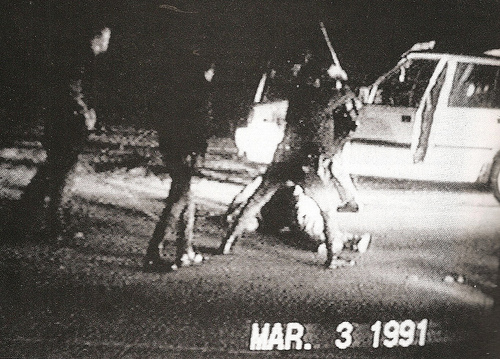
\includegraphics[width=0.4\textwidth]{figure/rodneyking.jpg}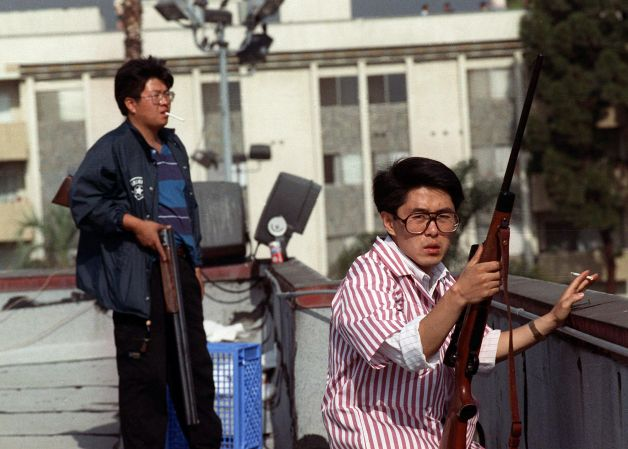
\includegraphics[width=0.4\textwidth]{figure/koreangrocer.jpg}\\
%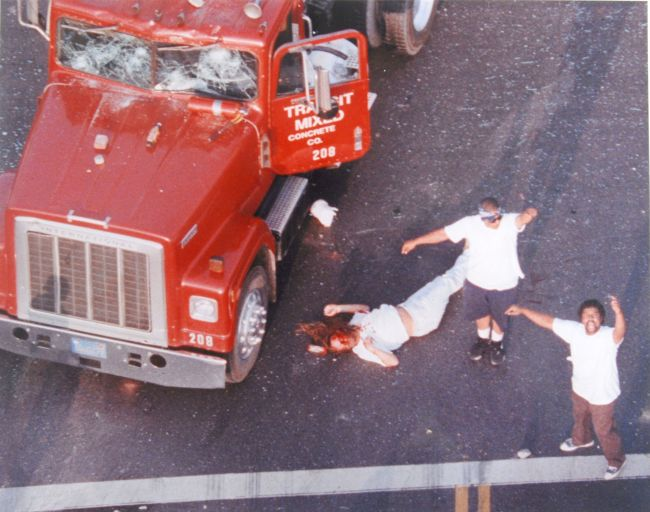
\includegraphics[width=0.4\textwidth]{figure/ReginaldDenny.jpg}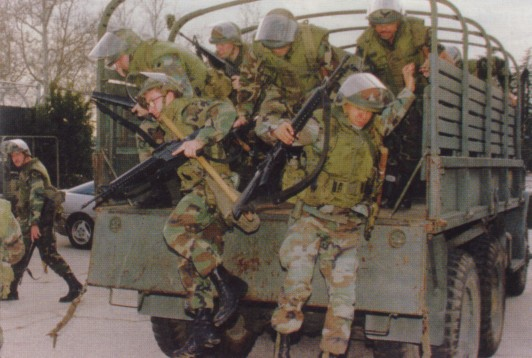
\includegraphics[width=0.4\textwidth]{figure/nationalguard.jpg}
%\end{center}
%
%\end{frame}
%%------------------------------------------------------------------------------
%
%
%%------------------------------------------------------------------------------
%\begin{frame}[fragile]
%\frametitle{Early 1990's Los Angeles}
%Then in 1994 there was a trial involving former NFL star O.J. Simpson.  He was accused of killing his ex-wife Nicole Brown Simpson and her friend Ron Goldman and later acquitted.  
%
%\begin{center}
%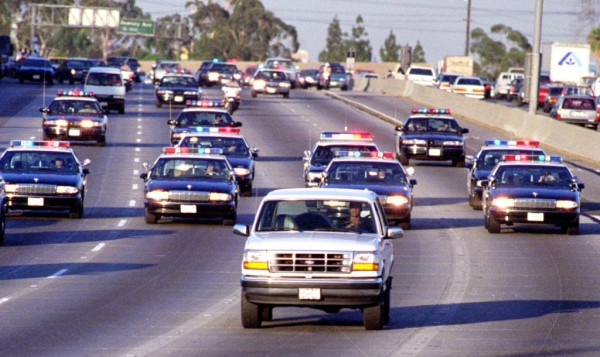
\includegraphics[width=0.6\textwidth]{figure/bronco.jpg}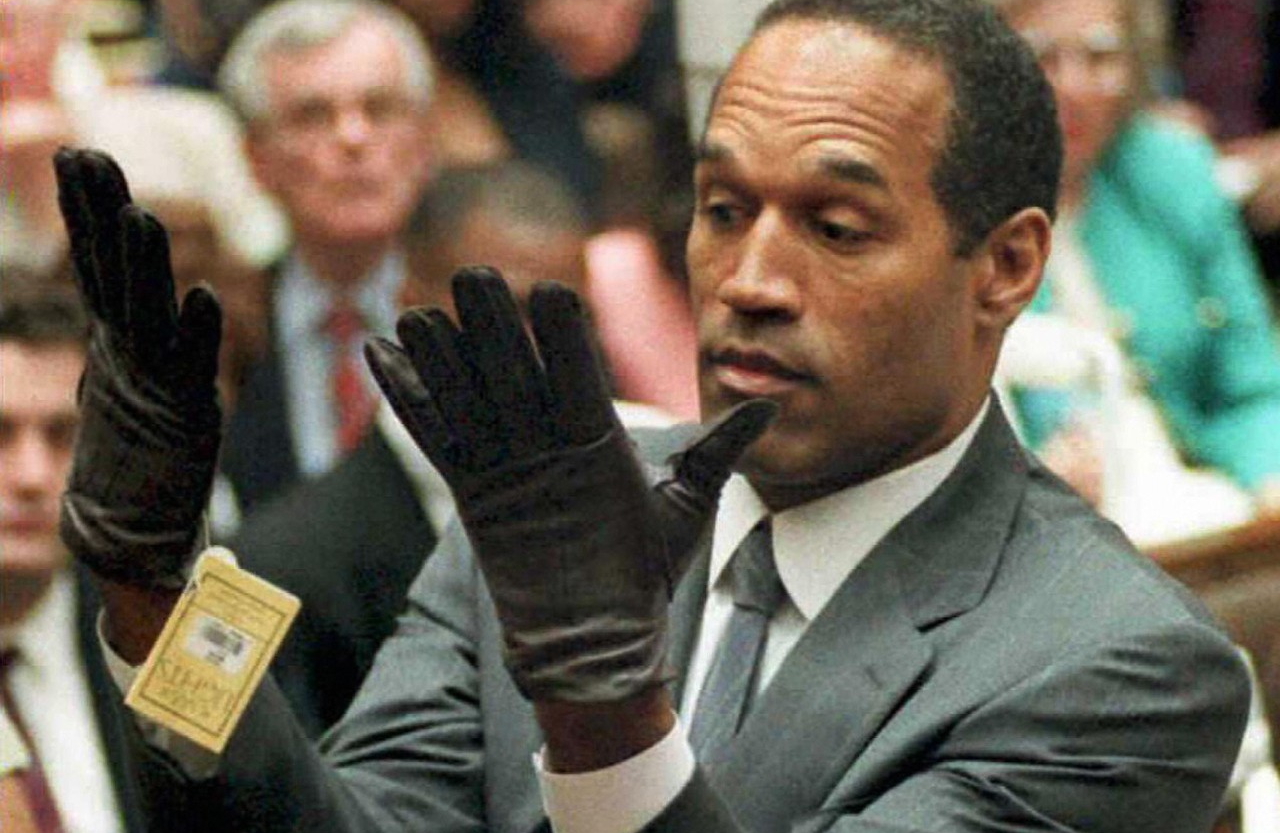
\includegraphics[width=0.4\textwidth]{figure/OJsimpson.png}
%\end{center}
%
%\end{frame}
%%------------------------------------------------------------------------------


%------------------------------------------------------------------------------
\begin{frame}[fragile]
\frametitle{Jury Selection}

In both sensational trials a big issue was the \blue{racial makeup} of the jury.  

\vspace{0.5cm}

\pause The question we ask is: is there a way to figure out if there is a \blue{racial bias} in jury selection?  

\end{frame}
%------------------------------------------------------------------------------


%------------------------------------------------------------------------------
\begin{frame}[fragile]
\frametitle{Jury Selection}
Say we have a population where the racial breakdown of the juror pool (registered voters) is:


\begin{center}
\begin{tabular}{l||cccc|c}
Race & White & Black & Hispanic & Other & Total \\ 
\hline
Registered Voters & 72\% & 7\% & 12\% & 9\% & 100\%\\ 
\textcolor{white}{Representation} & \textcolor{white}{0} & \textcolor{white}{0} & \textcolor{white}{0} & \textcolor{white}{100} & \textcolor{white}{$n=100$} \\ 
\end{tabular}
\end{center}


\end{frame}
%------------------------------------------------------------------------------


%------------------------------------------------------------------------------
\begin{frame}[fragile]
\frametitle{Jury Selection}
Say we had $n=100$ people picked as jurors, we \blue{expect} the breakdown to be:

\begin{center}
\begin{tabular}{l||cccc|c}
Race & White & Black & Hispanic & Other & Total \\ 
\hline
Registered Voters & 72\% & 7\% & 12\% & 9\% & 100\%\\ 
Representation & 72 & 7 & 12 & 9 & $n=100$ \\ 
\end{tabular}
\end{center}

\end{frame}
%------------------------------------------------------------------------------


%------------------------------------------------------------------------------
\begin{frame}[fragile]
\frametitle{Jury Selection}
Say we \blue{observe} the following breakdown.  Fairly obvious bias in juror selection!

\begin{center}
\begin{tabular}{l||cccc|c}
Race & White & Black & Hispanic & Other & Total \\ 
\hline
Registered Voters & 72\% & 7\% & 12\% & 9\% & 100\%\\ 
Representation & 0 & 0 & 100 & 0 & $n=100$ \\ 
\end{tabular}
\end{center}

\end{frame}
%------------------------------------------------------------------------------


%------------------------------------------------------------------------------
\begin{frame}[fragile]
\frametitle{Jury Selection}
But what about the following?  We expected 72 whites, but observe 75.  Is there a bias?  i.e. a non-random mechanism at play?

\begin{center}
\begin{tabular}{l||cccc|c}
Race & White & Black & Hispanic & Other & Total \\ 
\hline
Registered Voters & 72\% & 7\% & 12\% & 9\% & 100\%\\ 
Representation & 75 & 6 & 11 & 8 & $n=100$ \\ 
\end{tabular}
\end{center}

\end{frame}
%------------------------------------------------------------------------------


\end{document}










